\chapter{Introducing Social Navigation}
\label{chapter:social.navigation}

After we've descried how we collected our secondary literature for which we've
based this chapter, we'll briefly discuss navigation and sociality\dash{}both
in general terms and relating to the web. Then we'll concentrate on these two
topics together by looking at scholarly research where social navigation is
used consciously as a concept. By this we mean the research where either
social navigation is defined, redefined or problems relating to the concept is
discussed with a basis in such definitions.
We'll give an overview of social navigation and its concepts before diving in
to the various forms of social navigation that researchers have implemented
or proposed. In this latter section of applications of social navigation we'll
also include related examples from the real world where appropriate.
Finally, at the end of this chapter we'll briefly see if social navigation
can be valuable for navigation in web sites.

\enlargethispage{-\baselineskip}

\section{Literature Search}
\label{section:literature.search}

Before the literature search was conducted we did some preliminary thinking
about
\begin{inparaenum}[(i)]
  \item the focus of our topic to get more precise results, and
  \item what literature databases would yield sufficient and accurate
    findings.
\end{inparaenum}
Based on these concerns we settled on the literature indexes laid out in
\tablepageref{literature.databases} and used the following keywords%
\sidenote{
  With varying use of modifiers (i.e. \abbr{AND}) or quotations to find exact
  phrases
}
for search:

\begin{items}
  \iterm{social navigation} is the concept of our main topic.
  \iterm{collaborative filtering} is often used to realize our
    main topic.
  \iterm{recommender system} can be an application of our main topic.
  \iterm{tagging} can be related to our topic depending on use.
\end{items}

\begin{table}
  \begin{tabular}{ll}

    Type & \\

    \cmidrule(lr){1-1}

    Full-text &
    \abbr{ACM} Digital Library \\

    Bibliography &
    The Collection of Computer Science Bibliographies \\

    Reference &
    Inspec Online \\

    Bibliography &
    \abbr{HCI} Bibliography \\

  \end{tabular}

  \caption[Literature Databases]{Literature databases used for search}
  \label{table:literature.databases}
\end{table}

In addition to keyword based search we also conducted citation searches on the
articles that in our opinion seemed to be the most important in the field.
The articles that we found relevant during our literature search phase was
collected and studied. During this process we eliminated articles by the same
authors where similar topics and implementations were discussed and focused on
either the most recent or the most representative article.

\section{Navigation}
Navigation was traditionally associated with controlling a vessel at sea to
a given destination.%
\sidenote[-1]{
  \emph{Navigate} is in fact derived from the two Latin words \emph{navis}
  meaning \val{ship} and \emph{agere} meaning \val{to drive}
  \citep[\p{756}]{anderson97}.
}
Since then it's been used to describe behavior related to safely finding ones
way whether one is driving a car, flying a plane, or walking on foot. Maps
(a graphical representation of the medium one are navigating in)
and compass (a tool for connecting graphical maps to the physical world)
are often used as aids in this wayfinding.

When used in context of
computer systems navigation is essentially a metaphor of our usage of the
word in our physical world. Through computer systems we present users with a
conceptual space in which they can navigate \citep[\p{189}]{whiteside85}.
Today we normally present such a space as a \abbr{GUI}.%
\sidenote[-2]{
  \abbr{GUI} is short for graphical user interface. Our notion of a
  \abbr{GUI} was pioneered by \citet{sutherland63} and his
  \project{Sketchpad} system.
}

\subsection{Navigation on the Web}
\label{section:social.navigation.navigation.navigation.on.the.web}

The Web is based on the ideas of \term{hypertext}\dash{}a term coined by
\citet[\p{86}]{nelson65}. The essential part of hypertext are
\term{hyperlinks} \citep[\p{90}]{nelson65} which enables navigation between
distinct documents. While \citeauthor{nelson65} was clearly
inspired by the work of \citet{bush45} it has been argued \citep{rayward94}
that many of the features of hypertext was envisioned by Paul Otlet in his
\work{Trait\'e de documentation} of 1934.

Navigation is important on the Web. Without a way to efficiently and safely
navigate one is in danger of becoming lost. This problem was evident even
before the Web was invented as
\begin{fullquote}[\p{38}]{conklin87}{describes}
  Hypertext offers more degrees of freedom, more dimensions in which one
  can move, and hence a greater potential for the user
  to become lost or disoriented.
\end{fullquote}

\citet{jones96} studied the navigational support provided by the Web's first
browsers:
\begin{inparaenum}[(i)]
  \item loading of a page by entering its location,
  \item loading a bookmarked page,
  \item loading a page by using a hyperlink on the current page,
  \item recall previously visited pages with forward and backward buttons,
  \item recall a previously visited page by locating it in a history list, and
  \item reloading the current page.
\end{inparaenum}
While modern web browsers support more forms of navigation%
\sidenote[-7]{
  These early browsers' history lists were not remembered between sessions. In
  addition we're seeing browsers as \project{Flock} (available at
  \url{http://flock.com}) with new methods of navigation integrated.
  There is also an abundance of plugins and extensions for the main stream
  browsers which enable new possibilities for navigation.
}
than the earliest applications we're not concerned with those here.
We're only interested in the navigation which are conducted within the main
browser window (where web pages are rendered) enabled by following hyperlinks.
We can therefore define navigation on the Web for our purposes as:

\begin{quote}
  The behavior of clicking on a hyperlink in a web page.
\end{quote}

Following hyperlinks is
today the most used navigation method on the Web \citep[\p{10}]{weinreich08}.
\begin{fullquote}{garrett02}{%
  gives us a description of the physiology of such navigation which
  illuminates the thought process of the navigator}
    A typical user, faced with a typical, freshly loaded Web page\dash{}her
    eyes bouncing around the page\dash{}takes in all the options available.
    Maybe she scrubs the pointer over a few navigation elements. Then,
    finally, she's poised to click. In that moment, as her pointer hovers over
    the link and finger hovers over the mouse button, she has a picture in her
    mind of what is on the other end of that link.
\end{fullquote}

More specifically, we're either using a strategy of \term{browsing} or
\term{searching} when we're navigating the Web through hyperlinks.
\begin{fullquote}[\p{71}]{marchionini88}{%
  describes the characteristics of browsing}
    Browsing is an exploratory, information-seeking
    strategy that depends on serendipity. It is
    especially appropriate for ill-defined problems
    and for exploring new task domains.
\end{fullquote}
Serendipity\dash{}\openpostquote[\p{631}]{andel94}{%
  the art of making an unsought finding}%
\dash{}is what makes browsing effective as a navigation method in some
situations.
Search as a navigation method does not rely on serendipity as much as browsing
since you have a clearer idea about what you're navigating towards.

Today we often use search engines\dash{}either local to a particular web page
or global for all web pages\dash{}when
navigating the Web with a search oriented mind set.
\citet[\pp{53}{54}]{freyne07} distinguishes between browsing by navigating
with hyperlinks and searching by using a search engine. We've taken this
distinction and decided, as stated earlier, to only focus on navigation
through hyperlink usage. We'll therefore not look at search with search engines
as a form of navigation in our thesis.

\section{Sociality}

If one looks up the adjective \val{social} in the
\work{Oxford English Dictionary, second edition}
\prequote[\p{905}, \vol{15}]{simpson89}{it's defined as}{%
  capable of being associated or united \emph{to} others}
Discussion about explicit social matters is left for scholars of the social
sciences. We've therefore briefly introduced the term and are more concerned
with situations where it relates to computer systems. More specifically
we're going to look at sociality on the Web.

\subsection{The Social Web}
\label{section:social.navigation.sociality.the.social.web}

Sociality has become an integral part of our modern age version of the Web.
We called this generation of the web for \term{Web 2.0}%
\sidenote{%
  Web 2.0 was first used as the name of a conference arranged by
  O'Reilly Media. The \val{2.0} part of the conference name was then used to
  signify the revival of interest in the web after the dot-com bubble in the
  early 21st century \citep{oreilly07}.
  Later the founder of O'Reilly Media, Tim O'Reilly, defined
  the term as the characteristics of the web sites that survived the dot-com
  bubble and the web sites he deemed to be the best newcomers to the
  field \citep{oreilly05}.
}
in our introductory chapter. When \citet{oreilly05} introduced the term he
emphasized the characteristics of interaction, community, and openness.
But different people give Web 2.0 various meanings and there is no
established definition as
\begin{fullquote}[\p{15}]{treese06}{have experienced}
  Pinning down Web 2.0 is like trying to scoop up water with your hands. You
  can't really hold onto all of it, but after most of the water runs through
  your fingers, there's still something left.
\end{fullquote}

Some have synonymized Web 2.0 with the various types of systems on the
Web which have been popular in the recent years. Examples of such systems
are wikis, social network sites, folksonomies, mash-ups, blogs, and
syndication \citedouble{\paras{2.10}{2.24}}{beer07}{\pp{35}{37}}{murugesan07}.
But Web 2.0 is not a class of systems \citep[\p{28}]{millard06} even though
these examples often live up to the aspirations of interaction, community,
and openness embodied in Web 2.0.

We're sympathetic with the view of defining
Web 2.0 more by the attitude it has for enabling user participation for all
people \citep[\p{101}]{lin07} as the Web is becoming democratized
\citep{graham05}. This shift is concerned with both social and
technical factors as certain technology had to be in place for building
products that adheres to the principles of Web 2.0. We do however think it's
beneficial to use some examples of systems when describing Web 2.0 as a term.
We'll now look at several of these examples of Web 2.0 systems and
the more general characteristics, both social and technical,
of the Social Web.

\removeline

\subsubsection{Improved interaction}
One can argue that the most important
technological change related to interactiveness since the Web's infancy was
when \citet{garrett05} introduced \abbr{AJAX}.%
\sidenote[-12]{
  \abbr{AJAX} is an acronym for Asynchronous JavaScript and \abbr{XML}
  and was introduced as a term in 2005 \citep{garrett05}. It captures how
  modern applications on the Web uses JavaScript for retrieving data
  asynchronous  with the \code{XMLHttpRequest} object found in most recent
  web browsers. \abbr{XML} was then exemplified as a possible data-interchange
  format for the asynchronous requests. It's not a technical term but
  describes how a suite of technologies can be used together to create
  interactive web pages. In  addition to the technologies mentioned above one
  commonly use standardized markup and presentational languages for presenting
  information and JavaScript to not only fetch data, but enable behavior
  \citep[\p{282}]{stamey06}.
}
More elaborate interaction due to technological advances such as \abbr{AJAX}
enables production of applications on the Web previously only viable to
implement as desktop software \citedouble{\p{101}}{lin07}{\p{44}}{mesbah07}.
We're now able to create systems just like we've done on the desktop for 25
years, only in a different medium \citep[\p{64}]{arnowitz07}.
Interestingly, support for the core technical feature of \abbr{AJAX} was
introduced in March 1999 when \project{Microsoft Internet Explorer 5}
was released \citep{microsoft99}. It would still take almost six years before
such technologies saw such widespread use that a new term was warranted.

One possible reason for the lack of early developer uptake of this new
technology could be the disparate field of browser implementations.
Different browsers have variations in their interfaces for interacting with
web documents through JavaScript.%
\sidenote{
  For more about JavaScript, a programming language often used to implement
  behavior in web browsers, see
  \sectionref{selection.stack.client.language}.
}
It's quite hard to implement an application
when one have to write your code to handle several differences in browsers.
The JavaScript web platform have been described as
\postquote{crockford07}{%
  a really hostile programming environment}
\abbr{AJAX} comes with a price. One have to be quite proficient in the
intricacies of each browser to develop truly cross-browser applications.
Thankfully frameworks that abstract away such tediousness have come to
the rescue \citep[\p{45}]{mesbah07}. We believe part of the flourishing of
\abbr{AJAX} technologies are due to frameworks' ability to make browser
development friendly for the average programmer. At the moment of critical
mass \abbr{AJAX} hit a tipping point and the usage and uptake changed
dramatically similar to the way an epidemic spreads
\citep[\pp{8}{12}]{gladwell02}.

\subsubsection{Social network sites}
\label{section:social.navigation.sociality.the.social.web.social.network.sites}
Community brings the social aspect to the Web. While social
interaction on the Web is nothing new, greater availability for all
citizens of the Web to take part in such interaction is.

\begin{fullquote}{boyd07}{%
  give their definition of a \term{social network site} as}
    web-based services that allow individuals to (1) construct a public
    or semi-public profile within a bounded system, (2) articulate a list of
    other users with whom they share a connection, and (3) view and traverse
    their list of connections and those made by others within the system.
\end{fullquote}

The first site that adhered to \citeauthor{boyd07}'s definition was arguably
\project{SixDegrees}, which saw the day of light in 1997.%
\sidenote[-20]{
  SixDegrees closed their operations in 2000. Its founder believes SixDegrees
  simply was ahead of its time \citep{boyd07}.
}
There had been web sites that implemented
parts of this definition of social network sites, but SixDegrees was the
first to include all necessary characteristics.

The three most influential social network sites until this point of time
have been Friendster,%
\sidenote[-19]{
  Available at \url{http://friendster.com}.
}
MySpace,%
\sidenote[-17]{
  Available at \url{http://myspace.com}.
}
and Facebook%
\sidenote[-15]{
  Available at \url{http://facebook.com}.
  For the social navigational characteristics of Facebook look, at
  \sectionref{analysis.facebook}.
}
according to \citet{boyd07}. We feel this holds true if
one have an American world view.%
\sidenote[-12]{
  Blink (\url{http://blink.dagbladet.no}) for instance was a popular
  social network in our home country, Norway, before Facebook became
  adopted by Norwegians.
}
Friendster made some blunders by not listening to its users'
wishes and are therefore not widely used today. MySpace was launched in
2003 hoping to attract unsatisfied Friendster users \citep{boyd07}.
They were successful in this endeavor in addition to attracting loads of
music bands and later teenagers.
Facebook seems to be the hot social network today%
\sidenote[-12]{
  Facebook is now the largest social network site in our home country, Norway.
  As of May 14, 2008 it had approximately 1,142,300 registered profiles
  from Norwegian users.
  If every profile represents a unique individual (highly unlikely)
  this would mean that almost a quarter of all Norwegians are registered at
  Facebook. Data was collected by starting to register an advertisement for
  all Norwegian members and capture the market reach statistics.
  Population data was gathered from Statistics Norway (\url{http://ssb.no}).
}
attracting users from many walks of life.

\subsubsection{Mash-ups}
Openness enables exchange of information between
different parties so that new services on the Web easily can be created.
This phenomenon, a \term{mash-up},%
\sidenote[-2]{
  The term mash-up is taken from the similar activity finding place within the
  music scene where artists combine the music from one song with the
  \latin{a capella} from another song \citep{wikipedia08mashup}.
}
occurs when information and/or functionality from separate web sites and
services are brought together in a complementary way
\citep[\p{36}]{murugesan07}.

Mash-ups is most often created by utilizing one or more web \abbr{API}s.%
\sidenote[1]{
  \abbr{API} is short for Application Programming Interface and can be seen as
  a \postquote[\p{2}]{jacobsen91}{%
    set of calling conventions defining how a service is
    invoked through a software package}
}
\citet[\p{86}]{floyd07} argues that web \abbr{API}s enable innovation since
they provide access to robust technologies and massive amounts of
content\dash{}something no individual could create for himself. In addition
these \abbr{API}s lowers the barriers to entry since they often provide a
sound and efficient interface to content. Before the days web \abbr{API}s were
commonplace developers would resort to scraping web sites for getting a hold
of data. Even though such scraping still happens today, it seems that web
\abbr{API}s are proliferating.

\subsubsection{Collective intelligence}
The notion of \term{collective intelligence} is important for understanding
the characteristics of our modern web. It's been argued that the sharing we're
seeing in blogging, Wikipedia,%
\sidenote{
  Wikipedia\dash{}the free content encyclopedia allowing submissions from
  everyone\dash{}can be found at \url{http://en.wikipedia.org}.
}
and mash-ups
\postquote[\p{23}]{weiss05}{%
  could lead the way to a truly democratic network, where producers and
  consumers are one and the same}
This change is however not only technological, it represents a fundamental
mind shift \citep[\p{206}]{kolbitsch06}.
Collective intelligence is not unique
to the Internet but the communication facilities enabled by this relatively
new technology have created new ways for widely dispersed people to work
together \citep{mitcenter08}. The result is a lower barrier to entry for
taking part in a collaborative process where a shared intelligence emerges.

Collective intelligence is closely related to
\term{wisdom of crowds}\dash{}a phenomena that describes the amount of
information contained in a group's collective verdict.
In many situations the crowd is able to hold a complete picture of the world
in their collective brains \citep[\p{11}]{surowiecki04}. The larger the
crowd, the more accurate their answers will be.%
\sidenote[-4]{
  Take for example the Google search engine which we've now grown accustomed
  to use in our daily search because of the accuracy of the results it
  provides. The underlying principle of Google's search algorithm called
  PageRank is that a page is rated of importance based on how many pages who
  link to that page and the importance of the pages that linked there
  \citep[\p{109}]{brin98}.
}
A wise crowd is characterized by diversity of opinion, independence,
decentralization, and aggregation \citep[\p{10}]{surowiecki04}.
\citet{powazek08} argues that one have to design for selfishness to make
collective intelligence work in a community. If an individual don't have
self-interest in contributing knowledge, it will seldom happen.
\prequote{powazek08}{therefore sees collective intelligence as}{%
  selfish behavior aggregated for the common good}

In the case of Wikipedia, \citet{giles05} found a sample of science articles
to be comparable in accuracy to similar articles in
\work{The New Encyclop\ae{}dia Britannica}. While the quality of content in
these two sources was similar, readability and structuring of content seemed
to be better in the professionally edited encyclopedia.
\citet{lanier06} argues that while Wikipedia can be accurate it lacks
personality and context. In his view it's important to know whom the author is
and in what setting information is written.

\citet{lanier06} goes on to questioning the resurgence of collectivism on the
Web, not just in Wikipedia.
He thinks the reason for people's blindly usage of collectivism is happening
since bad old ideas packaged in modern technology have an confusing ability to
appear fresh. Just as individuals can be either
stupid or intelligent he feels the collective can be both stupid in some cases
and intelligent in others. Both individual and collective intelligence is
important since these two forms seems to not be intelligent in the same
settings.

\begin{fullquote}{lanier06}{%
  offers a set of conditions that have to be in place for enabling the
  collective to be smarter than the individual}
    The collective is more likely to be smart when it isn't defining its own
    questions, when the goodness of an answer can be evaluated by a simple
    result (such as a single numeric value), and when the information system
    which informs the collective is filtered by a quality control mechanism
    that relies on individuals to a high degree.
\end{fullquote}

Taking the advice of \citeauthor{lanier06} we have to question the answers
the collective gives us by providing structure and constraints and firstly
rely on intelligent individuals.

\section{Social Navigation}
\label{section:social.navigation.social.navigation}

Drawing on the previous explanation of navigation and definition of social, we
can combine the two terms. Social navigation then means going from one point
to another in a medium with other people.

Social navigation as a term was introduced in an article by
\citet{dourish94} where they discussed three types of navigational mechanisms,
spatial, semantic,%
\sidenote{
  \work{Oxford English Dictionary, second edition}
  defines the adjective \emph{semantic} as
  \postquote[\p{939}, \vol{14}]{simpson89}{%
    Relating to signification or meaning}
  Semantic navigation on the Web is navigation when one utilizes the semantic
  properties of hyperlinks and the semantic relationships amongst them.
}
and social, which they argue can be separated even though
there is evidence of situations where the different mechanisms are combined.
In their description of the social type of navigation
\begin{fullquote}[\p{1}]{dourish94}{%
  coined the term \term{social navigation}}
    When navigable information systems are extended to support collaborative
    activity, a third model of navigation arises. This is \emph{social}
    navigation. In social navigation, movement from one item to another is
    provoked as an artifact of the activity of another or a group of others.
\end{fullquote}

\citeauthor{dourish94} exemplifies two cases where neither location
(spatial) nor content (semantic) is used for exploration\dash{}the social
model is used on its own. Based on these two experiences
\citeauthor{dourish94} argues that we possibly need to move away from spatial
models of navigation and rather focus on designing explicitly with semantic
and social navigational techniques.

\citeauthor{dieberger97} highlights an important aspect for making interaction
on the Web smoother. With an
\openpostquoteyear[\p{812}]{dieberger97}{%
  awareness of the presence of other users}
one can give an indication of what parts of a web page that is of high demand
and possibly identify the users accessing them. This means that one can move
in the direction others are heading\dash{}one can follow the stream.

\citet[\p{39}]{dieberger00b} include the properties of \term{personalization}
and \term{dynamism} into their understanding of what social navigation is.
Social navigation is not pre-planned, but grown dynamically in an organic
fashion. This distinction is shown by the example of walking down a road in a
city versus walking on a forest trail. Personalization means that the
navigation advice is given to the receiver in a fashion that suits him.
Related to dynamism is social navigation's temporal nature.
\citet[\p{39}]{dieberger00b} shows this with the analogy of a forest trail
which will vanish if it's not used. This idea was envisioned for computer-like
systems by \citeauthor{bush45} over half a decade ago in that
\postquoteyear[\p{106}]{bush45}{%
  trails that are not frequently followed are prone to fade, items are
  not fully permanent}

\citet{svensson05} argues that while social navigation is plentiful in
our everyday world it's not implied that it's a good idea to implement
computer based systems with this perspective in mind. Instead of creating
translations from our physical world to our virtual world
they explain that one instead have to
\postquoteyear[\p{377}]{svensson05}{%
  make information spaces afford social interactions and accumulate
  social trails}
With \term{social trails} the authors mean traces left in the system by past
users guiding current users' navigational behavior.

\citeauthor{robins02} on the other hand argues that one can not rely on
technological structures alone when using social navigation which
\postquoteyear[par.~50]{robins02}{%
  transforms a space on a computer network into a virtual place}
During an ethnographic study the author examined social navigation in relation
to the persistent structures found in the physical world during a distance
education program. She found that these real world structures supported and
afforded social navigation in virtual places.

\subsection{Definition}

The most detailed definition of social navigation to our knowledge is
given by \citet{svensson03} in his Ph.D. thesis. To understand his
definition we'll have to introduce his nomenclature for the actors in a social
navigation process:

\begin{items}
  \iterm{The navigator} is \postquoteyear[\p{20}]{svensson03}{%
      the person seeking navigational advice}
  \iterm{The advice provider} is a \postquoteyear[\p{20}]{svensson03}{%
      person or artificial agent providing navigational advice to a navigator}
\end{items}

Social navigation was then defined by
\begin{fullquote}[\p{20}]{svensson03}{as}
  \dots navigation that is conceptually understood as driven by the actions
  from one or more advice providers.
\end{fullquote}

Firstly, \citeauthor{svensson03} talks about navigation which is
\q{conceptually understood} as driven by these advice providers. As long as
the user believes his navigational choices are driven by advice providers it
is social navigation. Secondly, the actions that the navigator is driven by
need not be only direct advice from a single advice provider, but can also be
aggregated of nature.

\subsection{Fundamental categorization}
\label{section:social.navigation.fundamental.categorization}

We'll take a look at broader characteristics of social navigation
before we'll continue with a discussion of several technical applications of
social navigation found in secondary academic literature.

\subsubsection{Active, direct, passive, \oldand indirect social navigation}

In his classic article \citet{dieberger97} distinguishes between
\term{active social navigation} and \term{passive social navigation}.
Such a distinction is grounded in the nature of the exchange of information
between the two parties involved in a social navigation process.
These are the advice provider\dash{}the creator of navigation
cues\dash{}and the navigator:

\begin{items}
  \iterm{Active} social navigation finds place when a person either
    deliberately seeks out another and asks for a navigation advice or
    intentionally gives away such navigational advice.
  \iterm{Passive} social navigation happens when people make available
    navigational aids that later can be used by another person.
\end{items}

\citeauthor{svensson03} groups navigation of a social type in
\term{direct social navigation} and \term{indirect social navigation}:

\begin{items}
  \iterm{Direct} social navigation occurs when
    \postquoteyear[\p{21}]{svensson03}{%
      communication between navigator and advice
      provider is mutual and two-way}
  \iterm{Indirect} social navigation is where
    \postquoteyear[\p{21}]{svensson03}{%
      communication between navigator and advice provider
      is non-mutual and in one direction}
\end{items}

Despite \citeauthor{svensson03}'s more precise wording, active social
navigation is similar to direct social navigation. Both are differentiated
with passive social navigation which is similar to indirect social navigation.
\citeauthor{dieberger97} characterizes the relationship between the
navigator and advice provider. \citeauthor{svensson03} on the other hand
describes the nature of the communication between the two parties.

\subsubsection{Explicit \oldand implicit advice}
\label{section:social.navigation.fundamental.categorization.explicit.implicit}

Related to passive or indirect social navigation is the notion
of \term{explicit feedback} and \term{implicit feedback}.
These terms can be used for distinguishing how
passive or indirect social navigation is provided by an advice provider.
Collecting advice given by an advice provider explicitly means that
the advice provider have to use conscious effort to make the advice available.
Such an advice provider can for instance choose to share an interesting web
site and does so by putting a hyperlink to it on his web page.

When advice is mediated implicitly the process for so doing are transparent
and unobtrusive for the advice provider. Based on the work the advice provider
would have done regardless of the social effects it conveys one can provide
advice to future navigators. An example of such behavior is recording of
browsing history that can be computationally evaluated to provide advice for
others. We'll return to such recording of history in
\sectionref{social.navigation.applied.forms.interaction.history}.

Active and direct social navigation inherently make advice available by
explicit feedback. Partaking in these direct methods of social navigation
will always require conscious effort by the advice provider.

\section{Forms of Social Navigation}

Social navigation have been applied in various forms described in
academic literature. What follows is a review of these forms of social
navigation sprinkled with examples from our modern web.

\subsection{Hyperlink sharing}

\citet{dieberger97} is particularly concerned with making handling of
\abbr{URL}%
\sidenote{
  Uniform Resource Locator. \abbr{URL} was formerly an abbreviation of
  Universal Resource Locator.
}
entities transparent for users both in the operating system and in various
tools related to web browsers. Making \abbr{URL}s invisible to users will in
his opinion enable more widespread use of social navigation through pointer
sharing. Web browsers handles \abbr{URL}s embedded as hyperlinks
transparently,
so we're not going to elaborate on matters of \abbr{URL} handling in
auxiliary systems here.

Both \cite{dourish94} and \cite{dieberger97} observed social navigation
activity on the Web when hyperlinks were shared on web pages.
Creators of these pages often had a list of pointers to other web pages.
These were the pointers they deemed interesting enough to actually go
through the trouble of creating such a listing for. By doing this they created
an opportunity for navigation based on social factors.

While pointer pages still is in existence, it seems that the increasing
use of blogs (see \chapterref{introduction} for details)
have resulted in a new form for sharing interesting web pages,
which often is other blogs. So called \term{blogrolls} is a way for blog
authors to list other blogs they are reading regularly. They thereby function
\postquote[\p{3}]{marlow07}{%
  as a navigation tool for readers to find other authors with similar
  interests}
An example of a blogroll can be seen in \figureref{scrsh.dailykos.blogroll}.

\sidefigure[Blogroll]{%
  Blogroll for Daily Kos,
  retrieved December 5, 2007, from
  \url{http://www.dailykos.com/}.
  Daily Kos is one of the most popular American collaborative
  political blogs where people provide news and opinion from a
  liberal point of view.
  \label{figure:scrsh.dailykos.blogroll}
}{%
  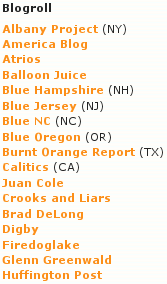
\includegraphics[width=0.8\marginparwidth]{scrsh_dailykos_blogroll}
}

\subsubsection{Social bookmarking}

A new phenomena appeared to the mainstream with the introduction of the
\project{del.icio.us}%
\sidenote[16]{
  Initially a system for organizing Joshua Schachter's personal bookmark
  collection, del.icio.us was introduced to a wider audience in 2003
  \citep[\p{223}]{livingston07}.
  del.icio.us is available at \url{http://del.icio.us}. 
}
\term{social bookmarking} system. This web site made individual
bookmark collections globally available, making it easy to discover what other
people was taking notice of. Interestingly \citet{keller97} created a system
in the early days of the web with almost the same features as social
bookmarking systems of today. This system, \project{WebTagger}, allowed
individuals to store bookmarks that later could be retrieved by other people.
The architecture of the system was based on a web proxy, which enabled
controls for storing the location of a given web page to be present within the
web page itself. Since the system was proxy-based, only users having enabled
the proxy server in their browsers could take advantage of the shared
bookmarks.

As \citet[\p{806}]{dieberger97} argues, the Web's growth\dash{}even at its
modest size in 1997 compared to its staggering size over 10 years
later\dash{}have implications on how easily it is to locate information.
By creating pointer
pages, and now socially shared bookmarking services, users are imposing a
structure on the web. By navigating these kinds of interlinked hyperlink
collections it's quite plausible that users are getting access to more highly
related and higher quality information. Sharing a hyperlink, either on you web
page or through a bookmarking service, requires a conscious effort. One would
believe that people only choose to do so for information they find
interesting.

\subsection{Tagging}

In addition to being a modern form of pointer pages, social bookmarking
with del.icio.us introduced a new way to annotate all kinds of
items.%
\sidenote[-1]{
  Like photos, articles, wine, books, videos, music, and so on.
}
By applying textual keywords to
bookmarks\dash{}and later other types of content\dash{}users were able to
browse such collections in new ways. These keywords have been popularized as
\term{tags} and the act of applying them is called \term{tagging}.%
\sidenote[-2]{
  Tagging was discovered by Joshua Schachter when he kept a plain text file
  with a list of all his web page bookmarks. He annotated these bookmarks by
  introducing single-worded labels prefixed with a number sign (\#). He could
  then easily search his bookmarks file with these labels by prefixing
  searches with the number sign. Schachter later introduced tagging to the
  masses by creating the del.icio.us social bookmarking site
  \citep[\p{92}]{weinberger07}.
}
Joshua Schachter, creator of del.icio.us, highlight tagging as its most
essential feature\dash{}the feature that set it apart from the competition
\cite[\p{225}]{livingston07}. Tagging solves a recurring problem with
using traditional folder or hierarchical categorization of items like
bookmarks. In such a system an item can only go in one folder. With
tags items can live in several categories at once
\citep[\p{93}]{weinberger07}.

The WebTagger system by
\begin{fullquote}[\p{1109}]{keller97}{%
  we described earlier had a novel approach to bookmark categorization}
    The system provides a simple means of organizing and sharing bookmarks
    using a structure-neutral categorization scheme, rather than a
    hierarchical filing scheme. The neutrality of this bookmarking scheme
    allows users to concentrate on tagging \abbr{URL}s with the most
    appropriate categories to facilitate subsequent retrieval, rather than
    forcing users to select a single best location within a rigid hierarchical
    structure.
\end{fullquote}

This description of the categorization scheme used in WebTagger very much
resemble tagging as found in del.icio.us. \citeauthor{keller97} even describes
the act of categorizing in this way as \emph{tagging}. While Joshua Schachter
may never have heard of WebTagger, it's evident that tagging was first used in
the WebTagger system\dash{}the first social bookmarking service.

\subsubsection{Folksonomy}

Tagging enables a user driven taxonomy (classification)
which is often called an \term{folksonomy}\dash{}a combination of the words
\emph{folk} and \emph{taxonomy}. A folksonomy is a strictly bottom-up
approach because of the lack of any predefined taxonomic structure.
Folksonomies therefore rely on \postquote[\p{31}]{marlow06}{%
  shared and emergent social structures and behaviors, as well as related and
  linguistic structures of the user community}
Since we're mainly interested in the navigational possibilities tagging can
give us, we're leaving out a deeper discussion of the benefits and drawbacks
of folksonomies.%
\sidenote[-7]{
  For those interested \citet{golder06} and \citet{marlow06} gives a detailed
  account of the tag usage and structure in respectively del.icio.us and
  Flickr\dash{}a social image sharing web site we dig deeper into
  when we analyze its social navigation capabilities in
  \sectionref{analysis.flickr}.
}

\subsubsection{Tag sharing \oldand scope}
\label{section:social.navigation.applied.forms.tagging.sharing}

As we've described tagging is often a collaborative process. Some web pages
for instance give suggestions for tags if the item you're annotating have
been tagged by others previously. Based on our own usage of collaborative
tagging system we seem to be more inclined to use some or all of these tags
than to come up with our own. In other words, our vocabulary is influenced
by the user community. \citet[\p{186}]{sen06} confirmed our personal
observations when they found that the community influence affects the
vocabulary of tags an individual uses. \citet[\p{355}]{farooq07} conducted
similar studies on a collaborative tagging service where the user interface
did not display the tags other people had applied for a similar resource.
They did not find any significant reuse of tags from other users and explained
this discrepancy with the lack of visualization of other user's tags while
tagging an item, as
evident in other bookmarking services. This means that one can influence
the vocabulary of users when they are applying tags by showing the
vocabulary of other users.

In addition to being shown other people's tags when tagging one can also
be given a list of the tags oneself have previously used.
Under such circumstances \citet[\p{185}]{sen06} found that the probability
of applying a previously used tag rose as the amount of tags the user had
applied increased. \citet[\p{355}]{farooq07} validated this phenomena
by showing similar results from another collaborative tagging system.

Applying your own tags for a given resource makes sense if you're annotating a
bookmark. You have your own representation of the bookmark given by the name
you gave it and the tags you have chosen to apply. Since a bookmark is
distinguished by a \abbr{URL} others can have other representations of the
same resource. For other content items as photos in a photo sharing site it
may make more sense to allow every user, not only the creator, to apply
globally visible tags for this single item. There is then only one
representation of this item and its tags.
Tags need not be collaboratively created. If for instance one are tagging
one's personal email messages it makes sense to keep such behavior private.

As we've seen folksonomies can be separated by their level of tag sharing:
private systems, fully open systems, and systems with user control over
what gets shared. In addition one can categoize folksonomies based on tag
scope: tags applied to an item globally
or belonging to separate users.%
\sidenote[-1]{
  For more about different characteristics of folksonomies see
  \citet[\pp{34}{36}]{marlow06} and their detailed account of such matters.
}

Annotating items seems to have benefits with regards to describing the items
and using them for categorization. But how does this relate to navigation?
By giving users a means to better describe various items it will hopefully be
easier for others to use this information in navigation\dash{}they will
hopefully more easily find the items or resources they are searching.

\subsubsection{Tag Clouds}

The seemingly most used way to display tags for navigation is by generating
a so called \term{tag cloud}.%
\sidenote{
  According to \citet{wikipedia08tagcloud} the first use of tag clouds
  was on Flickr for showing tags applied to photos. The idea of such
  visualization most likely came from \citet{flanagan03} in his display
  of search terms on his web site.
}
\begin{fullquote}[\p{1}]{fokker06}{%
  succinctly defines this visualization technique}
    The cloud is a representation of the frequency-based relation of tags.
\end{fullquote}

\begin{figure}
  
\includegraphics[width=\textwidth]{scrsh_tagcrowd_journal_redflavor}
  \caption[Research Journal Tag Cloud]{
    Tag cloud for the authors private research journal located
    at \url{http://journal.redflavor.com}.
    The tag cloud
    uses both font size and color to distinguish between
    the frequency of usage for the different tags.
    Generated with
    \project{TagCrowd} (\url{http://tagcrowd.com}) on May 12, 2008.
  }
  \label{figure:scrsh.tagcrowd.journal.redflavor}
\end{figure}

This means that a tag cloud is used to visualize how frequent various tags
are applied to one or more objects. Frequency is usually portrayed by varying
the font size based on usage. A highly utilized tag has a large font size
while less used tags have smaller font sizes. There are usually several levels
of font sizes in a tag cloud to visualize how popular tags are in relation to
others. Sometimes colors is used in addition to font size to even better
distinguish among the frequency of tag usage by showing the most used tags
with a higher contrast color than less used tags. Lastly tags are most often
listed alphabetically giving a visualization that in many ways resembles
clouds of various sizes in the sky.
\figurepageref{scrsh.tagcrowd.journal.redflavor}
shows an example of a tag cloud utilizing font sizes and color tones while
\figurepageref{scrsh.flickr.tagcloud} shows an example of a tag cloud using
only font sizes for distinguishing tags by frequency.

\citet[\p{996}]{rivadeneira07}
conducted a study of how varying properties of tag clouds affect
use. Unsurprisingly, font size had a large affect on how well a
given tag was perceived. Layout had a minor, but noticeable effect on
how well the users got an impression of the tag cloud.
\citet[\p{1314}]{halvey07} expanded on the findings by
\citeauthor{rivadeneira07} and found tag size to be important in how
fast information is found. During their study 
\citeauthor{rivadeneira07} also noticed that unalphabetized
tag clouds were inferior to alphabetized tag clouds when finding information.

\citet[\p{18}]{sinclair08} studied whether tag clouds provided
value for individuals seeking information through a folksonomy by making a
user interface which supported both search by keyword and navigation by tag
cloud. They found that a majority of users utilized the
tag cloud when looking for information \citeyearpar[\pp{22}{23}]{sinclair08}.
When looking for non-specific information\dash{}when the users were merely
browsing\dash{}this trend were even stronger. But for finding specific
information using  search by keyword required fewer queries than using tag
clouds \citeyearpar[\p{24}]{sinclair08}. \citeauthor{sinclair08}.
give merit to tag clouds as a navigational interface since it
reduces the costs of query\dash{}clicking is faster than typing and scanning
the tag cloud is faster than formulating a search query
\citeyearpar[\p{27}]{sinclair08}. The most important finding to take away from
this study is that tag clouds does not function well as the sole navigation
mechanism for folksonomies. Complementary navigation, with for example search
by keyword, needs to be in place for enabling efficient navigation.

\subsubsection{Tags as social navigation}

\citet{millen06} gives an account of how they used collaborative
tagging as a means for enabling social navigation in their
\project{Dogear} social bookmarking system. When users
were navigating bookmarks they most frequently browsed bookmarks for a given
user. But browsing by a tag was not much less frequent, supporting evidence of
the usefulness of folksonomies for enabling social navigation. In addition
it was found that of all bookmarks clicked, 74\% was of other user's
bookmarks. Such a high
\begin{sparkline}{3}
  %Name  Size  Unit
  %2005  100%  1 
  %2007   74%  .74
  \sparkspike .25  1
  \sparkspike .75  .74
\end{sparkline}
usage of other users' bookmarks was interpreted as a sign of high degrees of
social navigation within the system.

\subsubsection{Problems with tagging}

\citet[\p{1}]{fokker06} argues that social tagging is ideal in situations
where you have objects one can not easily perform keyword search on.
If such objects for instance are composed of video content, tags
can serve as an augmenter for performing keyword based searches as one can
do in textual content. They leveraged tagging in this manner when creating a
prototype of Wikipedia supporting video content\dash{}using tags as the
principle navigation mechanism. By doing so \citet[\p{2}]{fokker06}
saw the need for bootstrapping the availability of tags so that users would be
more inclined to create their own tags. Their solution was to algorithmically
create tags based on the textual contents of Wikipedia.
They hoped the existence
of these tags would stimulate users to start tagging themselves. Just as
social network sites have problems satisfying users before a
sufficient amount enrol, folksonomies have initial pains when
few annotations are available.

Tagging have further shortcomings. Tags could be misspelled, tags with the
same name are not always  homonymous, and tags with the same meaning does not
always have the same name because of synonyms \citep[\p{59}]{aurnhammer06}.

In addition \citet[\p{943}]{li07} argues that browsing tags by traditional
methods with keyword search or tag clouds is inefficient when the set of tags
are quite large. They implemented a system to mediate the synonymy and
homonymy problems with tags in addition the the problems with browsing a large
collection of tags. Their solution for tag ambiguity
was to generate the semantic concept%
\sidenote[-10]{
  Generating the semantic concept of a tag means to derive its meaning in
  a broader sense. Say for instance that a user is browsing for
  \emph{movies}. An algorithm that generates the semantic meaning of
  \emph{movies} could for instance map this to the concept of \emph{movie},
  where such tags as \emph{movies}, \emph{film}, and \emph{flick} could be
  associated with the concept of \emph{movie}.
}
of a tag and use that semantic meaning
when the user was looking for resources through tag browsing
\citep[\p{946}]{li07}.
As \citet[\p{95}]{weinberger07} argues, this problem
with tag ambiguity does not really matter when the collection of annotated
items becomes sufficiently large. One would only be concerned with such
matters if one need to find every possible item that is associated with a
concept.

The problem of browsing large scale tagging collections can be tackled by
inferring a hierarchy%
\sidenote[-8]{
  One can tag objects by several levels of abstraction. One can for instance
  tag a movie with \emph{movie} to identify what it is. Then one could use
  the tags \emph{comedy}, \emph{romanticcomedy}, and \emph{norwegian} for
  describing the object's features. One could computationally derive a
  hierarchy from the varying levels of abstraction in such tags saying
  that \emph{comedy} is the child of \emph{movie} and \emph{romanticcomedy}
  is the child of \emph{comedy}.
}
from the flat tag space \citep[\pp{946}{948}]{li07}.

\parabreak

We've seen that item annotation or tagging can be used to annotate items for
describing the information they convey and
thereby afford navigation. As we'll see in
\sectionref{social.navigation.applied.forms.recommendations}
annotations can also be used for describing the quality, importance, or
usefulness of an item and thereby potentially creating recommendations.

\subsection{Interaction history trails}
\label{section:social.navigation.applied.forms.interaction.history}

\citet{wexelblat99} contrasts the digital world of
computers with our physical world with respect to the formers lack of history.
In our traditional world we exploit such historical information traces
\postquote[\p{270}]{wexelblat99}{%
  to guide our actions, to make choices, and to find things of
  importance or interest}
It's argued that this apparent lack of history in computerized systems must
be sorted out such that future users can take advantage
of past users' historical traces left when they were working
on solving problems similar to the current user's.
A possible remedy for this problem on the Web is put forth in the authors'
\project{Footprints} system\dash{}a navigational aid as an extension to
normal web browsers. This navigational aid visualizes interaction history of
past users, enabling current users to navigate this history.
The interaction history consists of several navigation trails which are
\postquote[\p{273}]{wexelblat99}{%
  coherent sequences of nodes followed by an individual}

The idea of such trails of navigation far preceded \citeauthor{wexelblat99}
as they were envisioned by \citet{bush45} when he proposed the infamous
theoretical computer-like system named the \project{Memex}.%
\sidenote{
  The Memex was not envisioned as a computer system but as a
  mechanical system consisting of a set of controls hooked up
  to a microfilm reader and camera. It was
  theorized by \citeauthor{bush45} to be a system for handling
  a person's entire collection of documents, books, and communication.
  It was
  important that a user would be able to access this information with great
  speed and flexibility. An integral part of enabling such efficient access
  was a user' and content providers' ability to introduce trails between
  information items. \citeauthor{bush45}'s writing about trails
  inspired hypertext \citep[\p{86}]{nelson65} which in turn was the grand idea
  behind the World Wide Web \citep[\p{49}]{myers98}.
}
\citeauthor{bush45} describes a scenario where users are building trails
explicitly, inserts comments if needed, and gives it a name.
\citeauthor{wexelblat99} on the other hand
implemented a system where trails were automatically collected using a set of
heuristics to identify browsing behavior representing a coherent navigation
trail. These characteristics makes Footprints a passive and indirect social
navigation system.

\citeauthor{bush45} wrote his essay before the invention of computer networks
and he thinks of each Memex as a separate island. Sharing of trails is
possible through an exportation and following importation process, making it an
explicit action for its users.
The Footprints system makes the social process of sharing trails implicit and
transparent to its users\dash{}multiplayer is forced.

Controlled user studies by \citeauthor{wexelblat99} did partially falsify
their pre-test hypothesis of Footprint's ability to let users find more
relevant results in a more efficient manner during a specific browsing task.
Users of the history-enriched system reported significant lower values of mean
page count in their browsing tasks. No significant difference in the quality
of the located information was found between users of a
plain web browser and those with a browser enhanced with Footprints.
They also found people experienced in the problem domain of the browsing task
to a larger degree being able to take advantage of interaction history
compared to novices.
\citeauthor{wexelblat99} attributed this finding to experienced people's
ability to have a clearer mental model of the information they was browsing.

\project{Trailfire}%
\sidenote{
  Available at \url{http://trailfire.com}.
}
is a modern incarnation of some of \citeauthor{bush45}'s Memex ideas.
By installing a browser extension users can
create trails of web pages which are automatically shared with other users.
The difference between Trailfire and Footprints is that trail creation in the
former system is an explicit task while the latter system make this process
implicit. \figureref{scrsh.trailfire.trail} shows one web page in a trail
created with Trailfire. Each page in the trail gets an information box with
navigation controls for moving through the trail, in addition to information
about why this particular page was included in the trail.

\begin{figure}
  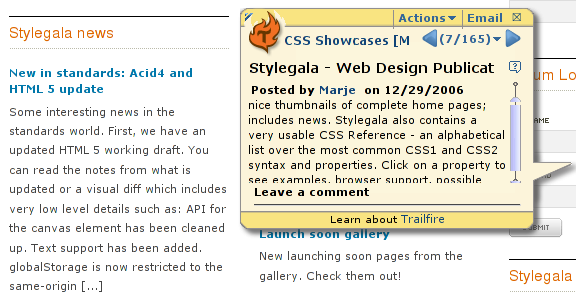
\includegraphics[width=\textwidth]{scrsh_trailfire_trail}
  \caption[Trailfire Trail]{
    Browsing a trail in Trailfire,
    retrieved May 22, 2008, from
    \url{http://trailfire.com/Marje/marks/37759}.
  }
  \label{figure:scrsh.trailfire.trail}
\end{figure}

\subsection{Collaborative filtering}
\label{section:navigation.applied.forms.collaborative.filtering}

\term{Collaborative filtering} \postquote[\p{175}]{resnick94}{%
  help people make choices based on the opinions of other people}
These choices are often used for navigation. Since the collaborative process
of creating opinions are of a social nature collaborative filters are a form
of social navigation.

The origin of the concept comes from the \project{Information Tapestry}
project where users could annotate electronic documents arriving in a
continuous stream\dash{}typically email messages \citep[\p{69}]{goldberg92}. By
installing a pre-existing filter, or creating one from scratch in a
special query language, users were able to filter out the essential documents
based both on explicit feedback through annotations and
meta-data concerning the document \citep[\p{62}]{goldberg92}.

\citet{resnick94} expanded on the ideas put forth in the Tapestry project
and created \project{GroupLens},
a system for collaboratively filtering Usenet postings. What was novel with
their approach at the time was that they could
\postquote[185]{resnick94}{%
  automatically determine how much weight to place on each
  evaluation, based on the degree of correlation between past
  opinions of the reader and evaluator}
This made the filter more personalized and would arguably give more
satisfying results. Such an approach gives a conceptual model where
\begin{inparaenum}[(i)]
  \item the user enters ratings which constitutes a profile
    for that individual,
  \item the collaborative filtering system finds
    the individuals with similar profiles\dash{}neighbors,
  \item the ratings of the user's neighbors are aggregated
    to form recommendations \citep[\p{243}]{herlocker00}.
\end{inparaenum}

During further studies of the GroupLens system \citet[\p{84}]{konstan97}
noticed some users' lack of incentive to rate content. Their solutions
was to introduce implicit ratings in addition to the existing explicit ratings
system.%
\sidenote{
  Implicit and explicit ratings reflect how the feedback is given by the
  advice provider as we've seen in
  \sectionref{social.navigation.fundamental.categorization.explicit.implicit}.
}
The implicit ratings were collected by monitoring whether a user read
an item, and for how long he kept reading it. Their initial studies showed
positive results for implicit ratings in that they were nearly as accurate as
explicit ratings. \citet[\p{39}]{claypool01} validated the results
\citeauthor{konstan97} experienced when they tested explicit and implicit
ratings against each other. \citeauthor{claypool01} found implicit ratings
to be somewhat less accurate than explicit ratings, but suggested implicit
ratings could be used successfully since they won't introduce the additional
overhead explicit ratings embodies.

Tapestry and GroupLens lacks a direct connection
between the advice giver and the navigator. Using the language of
\citet{dieberger97} they are both passive collaborative filtering systems.
\citet{maltz95} noticed how passive filtering systems required a
critical mass of users to be useful. They therefore created an active
collaborative filtering system.
\begin{fullquote}{maltz95}{%
  found circumstances where one of the two types of collaborative filtering
  systems offered better solutions}
    In \q{passive} collaborative filtering the system works better the higher
    the convergence of votes on the same set of documents. In contrast, the
    benefit of \q{active} collaborative filtering increases with the
    divergence of documents that are found.
\end{fullquote}

\citet[\pp{242}{243}]{herlocker00} gives compelling reasons for explaining to
users how the collaborative filtering process works. Usage experiments
showed explanations' ability to increase the acceptance of advice given by
collaborative filtering systems. Whether explanations improved actual
filtering performance was not certain\dash{}even though the authors
strongly believed in this idea
\citep[\p{250}]{herlocker00}.

Collaborative filtering is used on several modern web sites. One example is
\project{Reddit}\dash{}a web site where people can submit links to everything
they find interesting. Users of the community then votes these submissions up
or down (explicit advice) as one can see in \figureref{scrsh.reddit}.
Submissions are then
sorted based both on how many votes it have and how new it is. Users are not
given personalized listings based on their voting history. Reddit is thus
similar to Tapestry with regards to how the collaborative filtering works in
that similarities amongst users is not inferred (as in GroupLens).

\begin{figure}
  
\includegraphics[width=\textwidth]{scrsh_reddit}
  \caption[Collaborative Filtering at Reddit]{
    Collaborative filtering at Reddit, Stories can be voted up and down
    by using the up and down arrows. The first entry has been voted up by
    the author (the up arrow is highlighted red) which gave the submission
    a point, resulting in 132 points total.
    Retrieved June 25, 2008, from
    \url{http://reddit.com/r/programming}.
  }
  \label{figure:scrsh.reddit}
\end{figure}

As Reddit recently became open source%
\sidenote{
  The source code of Reddit can be found at
  \url{http://code.reddit.com}.
}
we were able to take a peek into its
collaborative filtering functionality. We did this to dissect how
collaborative filtering algorithms are used in real applications. The source
code of this algorithm can be found in
\sourcecodepageref{reddit.cf.algorithm}.
What follows is the algorithm used on Reddit in mathematical notation.

Given the time the entry was posted $t_{posted}$ and
the time of 7:46:43 a.m. December 8, 2005 $t_{cutoff}$,
we have $t_s$ as their difference in seconds
\begin{align*}
  t_s &= t_{posted} - t_{cutoff} \\
  \intertext{and $v_{sum}$ as the difference between the number of up votes
             $v_{up}$ and the number of down votes $v_{down}$}
  v_{sum} &= v_{up} - v_{down} \\
  \intertext{where the sign $s \in \{-1, 0, 1\}$}
  s &= 
  \begin{cases} 
     1 & \text{if } v_{sum} > 0 \\
     0 & \text{if } v_{sum} = 0 \\
    -1 & \text{if } v_{sum} < 0
  \end{cases} \\
  \intertext{and $v_{max}$ as the maximal value,
             of the absolute value of $v_{sum}$ and $1$}
  v_{max} &= 
  \begin{cases} 
    |v_{sum}| & \text{if } |v_{sum}| \geq 1 \\
    1   & \text{if } |v_{sum}| < 1
  \end{cases} \\
  \intertext{we have the rating as a function $f(t_s, s, v_{max})$}
  f(t_s, s, v_{max}) &= \log_{10}{v_{max}} + \frac{st_s}{45000}
\end{align*}

The resulting rating is a real number which is used for numerically sorting
entries. This is neither a computationally expensive algorithm nor a very
complicated algorithm. In spite of this we feel it delivers satisfying results
(as daily users of Reddit).

\parabreak

As we've seen, collaborative filtering is applied to generate
recommendations for users. These recommendations can aid users in navigating
towards content hopefully interesting for them.

\subsection{Recommender systems}
\label{section:social.navigation.applied.forms.recommendations}

\begin{fullquote}[\p{56}]{resnick97}{%
  clearly describes what a recommender system is}
  It is often necessary to make choices without sufficient
  personal experience of the alternatives.
  [\ldots]
  Recommender systems assist and augment this
  natural social process.
\end{fullquote}

What is then the difference between a collaborative
filtering system and a recommender system?
Recommender systems is a broader concept than collaborative
filtering. There are two ways a recommender system can generate
recommendations for its users:

\begin{enum}
  \item Using collaborative filtering
    where the verdicts of other users, which in some way are deemed to have
    similar taste as yourself, are used for recommendation\dash{}a social
    process.
  \item Using a \term{content-based} approach where one is relying on the
    nature of potential items instead of other people's perception of them.
    Based on your previous usage or reaction to items, similar items can then
    be recommended\dash{}an asocial process.
\end{enum}

The distinction between a content-based and collaborative filtering approach
lies in the way collaborative filtering \postquote[\p{241}]{herlocker00}{%
  are based on human and not machine analysis of content} To put it another
way the similarity of users are measured instead of the similarity of content.
Because of this distinction, collaborative filtering systems
and content-based systems have been called \term{user-based} and
\term{item-based} recommendation systems respectively
\citep[\p{156}]{greco04}.

Recommender systems can be based on either one or both of these approaches
\citep[\p{241}]{herlocker00}. \citet[\p{70}]{balabanovic97} argues that a
hybrid approach to recommendation is superior to an purely content or
collaborative solution since it
\begin{inparaenum}[(i)]
  \item enables one to use content-based recommendation for items
    not yet recommended by other individuals,
  \item enables one to use content-based recommendation when there are
    no other individuals with the same taste,
  \item when collaborative recommendations are present those can be
    used in favor of more imprecise content-based techniques, and
  \item collaborative recommendations can be generated even though users
    have not rated the same items by inferring such ratings through content
    similarity.
\end{inparaenum}
Since we're concerned with socially constructed navigation possibilities we're
not going to discuss content-based systems further in this thesis.

\subsubsection{Recommendation from tags}

One of the two forms of social navigation found in
\project{Knowledge Sea}\dash{}a digital educational
library\dash{}is recommendations by item
annotation \citep[\p{13}]{brusilovsky05}. Users can leave their emphatic marks
on content and thereby specify its usefulness. Questionnaires showed that a
fair majority of users was agreeable to the use of such recommendations
\citeyearpar[\p{15}]{brusilovsky05}. Analysis  of server logs strengthened
the impression
\begin{fullquote}[\p{38}]{brusilovsky05}{had by showing that}
  Social navigation support and specifically
  annotation-based social navigation increases the chance of
  accessing a resource dramatically.
\end{fullquote}

Advanced algorithms from the field of collaborative filtering
and recommender systems have been used together with folksonomies
consisting of collaborative tags
\citep[\pp{112}{113}]{wu06}. Preliminary studies have shown positive
results when harnessing such social knowledge with filtering algorithms
as opposed to traditional folksonomy representation
\citep[\p{114}]{wu06}.
Using a folksonomy for this purpose can hoverer interfere with an
existing recommender system. \citet[\p{190}]{sen06} found that the
introduction of tagging and tag display in their established
movie recommender system interfered with some of the users' primary
objective: finding interesting movies. Note that this dislike of
folksonomies was more likely to be present for users familiar with the old
movie recommender system sans a folksonomy. New users, having not
witnessed the recommender system without a folksonomy, seemed more
acceptant towards tagging.

But recommender systems have not only been extensively used in research
settings. Many of todays web sites uses some sort of recommender system to
deliver a better experience to their users. The canonical example is Amazon's%
\sidenote{
  An online store primarily carrying books at
  \url{http://amazon.com}.
}
usage of recommendations for book purchases. As seen in
\figureref{scrsh.amazon.recommendation}
Amazon deploys both collaborative filtering (similar people's purchases
determined by shared search history) and content-based recommendation (based
on personal browsing history).

\begin{figure}
  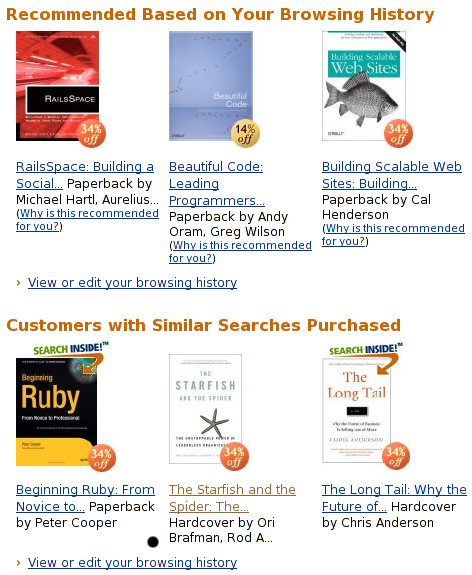
\includegraphics[width=0.90\textwidth]{scrsh_amazon_recommendation}
  \caption[Recommendations at Amazon]{
    Item-based and user-based recommendation at Amazon,
    retrieved May 21, 2008, from
    \url{http://amazon.com}.
  }
  \label{figure:scrsh.amazon.recommendation}
\end{figure}

In 2006 \project{Netflix}%
\sidenote{
  An online movie rental company located at \url{http://netflix.com}.
}
announced a contest where the first person to improve their existing
recommender system by 10\% would be eligible for a \$1 million prize
\citep[\p{1}]{segaran07}. By offering such a large reward Netflix
highlight how important accuracy in recommender systems can be for a company's
earnings. As of this writing no team has yet claimed the prize, but the front
runners from \abbr{AT\&T} Labs Research currently have a 9.12\% improvement
\citep{netflix08}. The secret to their recommender improvements was to employ
a variety of collaborative filtering methods and content-based methods.
A approach resulted in a situation where the different methods
complemented each other \citep[\p{4}]{bell07}.

\subsection{Social texture}

We use \term{social texture} to describe socially constructed annotations or
visualizations which may be used for navigation or in some form guide
users in navigational choices.

Social texture ties in with the forms of social navigation we've
recently discussed. Tagging, for instance, is a social texture. Tag clouds are
especially good examples of social texture.
The interaction history systems we've discussed uses forms of visualizations
in close proximity to hyperlinks to convey their degree of usage. This is also
a form of social texture.

The first forms of social texture used in computer systems (to our knowledge)
occurred when \citet{hill92} took advantage of
\term{computational wear}\dash{}an analogy for the
wear physical objects experience when being used. They modified a text
editor to show both wear related to document edits and readings of documents.
This wear was graphically visualized through the editor's scroll bar.
The concept of edit and read wear has since been used on the Web in for
instance the Footprints system \citep{wexelblat99}.

\begin{figure}
  \captionstyle{\raggedright}
  \begin{whole}
    \begin{minipage}[t]{0.475\wholewidth}
      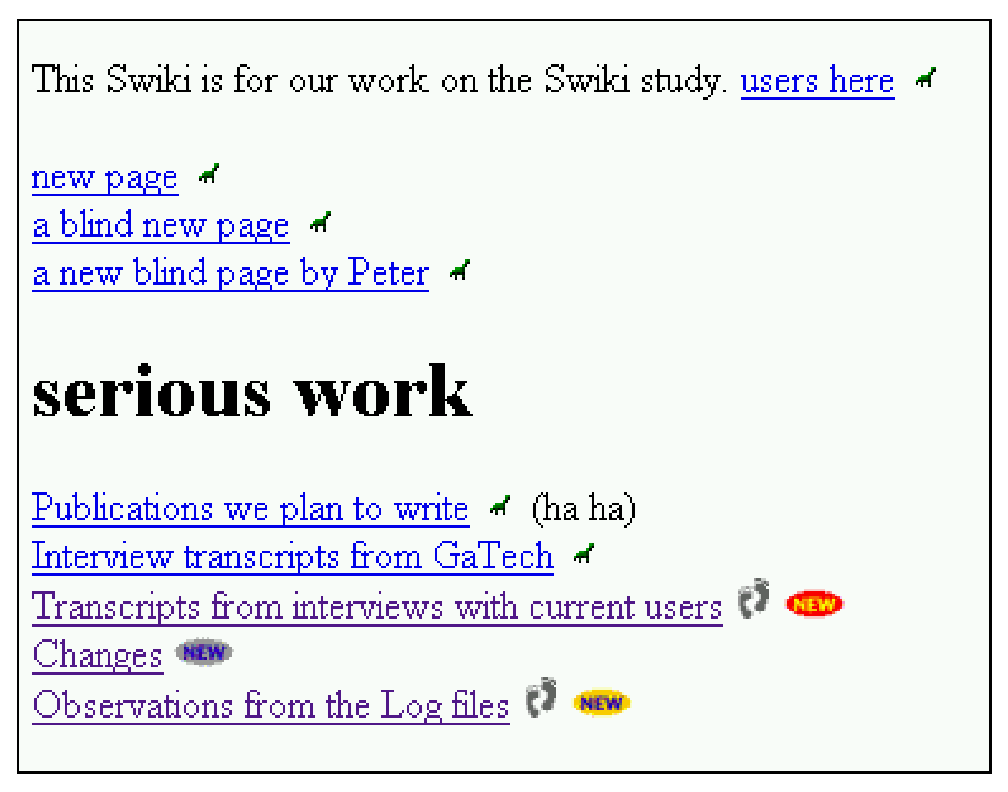
\includegraphics[width=\textwidth]{scrsh_coweb_contextual}
      \caption[CoWeb Contextual Cues]{%
        Contextual interaction history cues next to hyperlinks in CoWeb,
        retrieved January 25, 2008, from
        \url{http://homepage.mac.com/juggle5/WORK/publications/SwikiWriteup.html}.
      }
      \label{figure:scrsh.coweb.contextual}
    \end{minipage}
    \hfill
    \begin{minipage}[t]{0.475\wholewidth}
      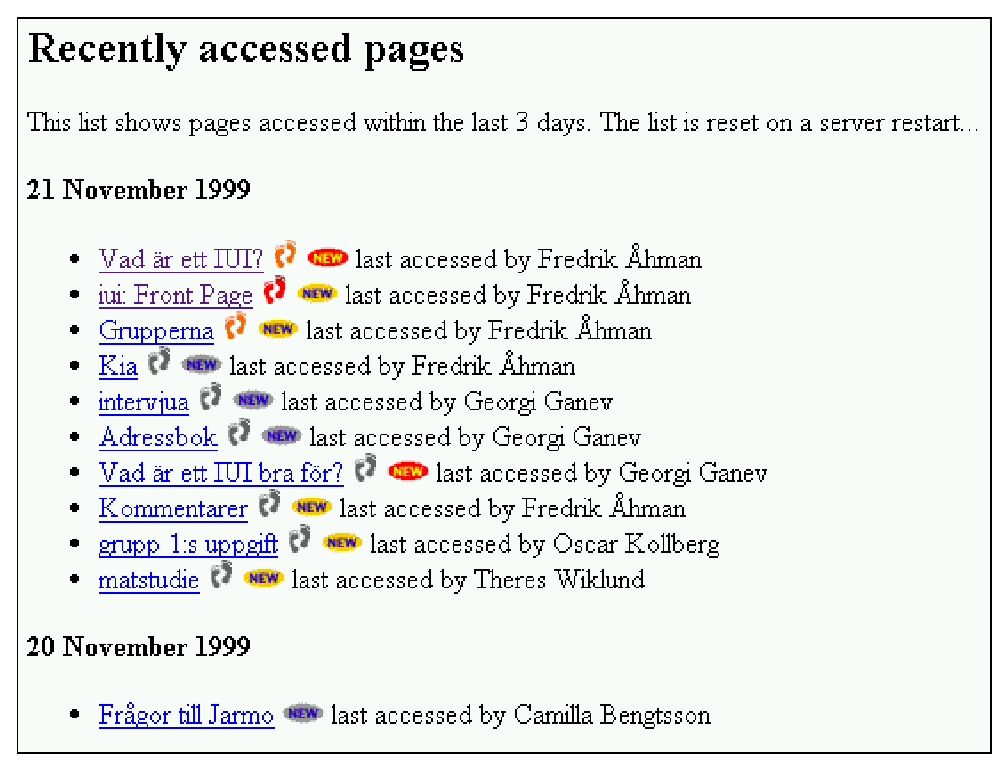
\includegraphics[width=\textwidth]{scrsh_coweb_global}
      \caption[CoWeb Global Cues]{%
        Global list of interaction history cues in CoWeb,
        retrieved January 25, 2008, from
        \url{http://homepage.mac.com/juggle5/WORK/publications/SwikiWriteup.html}.
      }
      \label{figure:scrsh.coweb.global}
    \end{minipage}
  \end{whole}
  \normalcaption
\end{figure}

\citet{dieberger00a} modified \project{CoWeb}\dash{}a collaborative Web space
modelled after Ward Cunningham's famous Wiki\dash{}to include interaction
history visualization hoping to make it a more social space, enabling social
navigation. They visualized other users' access of different pages both by
including a global list of such behavior and contextual cues about access
next to internal hyperlinks.
It was inferred by \citeauthor{dieberger00a} that markers of interaction
history increased the overall activity on the web page during a user study.
They also learned that it's important to provide both global and
contextual interaction history cues. Both
contextual and global use of such social texture can be seen in
\figureref{scrsh.coweb.contextual} and \figureref{scrsh.coweb.global}.

\citet{xu06} modified a Wiki in even more elaborate ways
with the aim of integrating several social navigational mechanisms.
They used read-wear information for creating social
texture in the Wiki both in-line pages, on a page level, and on a global
level. \citeauthor{xu06} took the approach of displaying read-wear in real
time, thus making the system look like a populated space. To make such an
approach useful the Wiki needs a certain amount of users present at all times.
If it's not frequently trafficked it would probably be better to represent
historical read-wear as done in CoWeb \citep[\p{220}]{dieberger00a}.

\project{virtPresenter} is a hypermedia based lecture viewer where read-wear
have been used to visualize a groups' interaction with continuous content
\citep{mertens06}. By following the traces other users have left current users
can interpret what's the most sought after parts of a lecture. The
visualization is implemented in ways similar to \citet{hill92} by showing
graphs of usage in line with a timeline selector and can be seen in
\figureref{scrsh.virtpresenter.timeline}.

We discussed KnowledgeSea regarding its use of recommendations in
\sectionref{social.navigation.applied.forms.recommendations}.
The system also incorporates what the authors calls
\term{traffic-based social navigation}
\citep[\p{12}]{brusilovsky05}\dash{}in other words history based
visualizations in the form of read-wear. The access of different articles in
the digital library are recorded and the degree of usage is then visualized in
the form of different color tones where darker indicates a more popular
resource. Such visualization is used consistently throughout the web site. A
questionnaire revealed that in excess of 70\%
\citeyearpar[p.15]{brusilovsky05} of the users
found such history based visualizations useful and appropriate.

\begin{figure}
  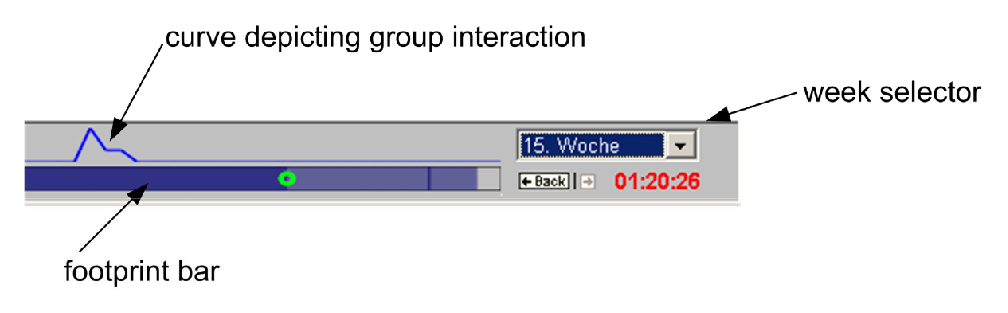
\includegraphics[width=\textwidth]{scrsh_virtpresenter_timeline}
  \caption[virtPresenter Timeline]{
    virtPresenter Timeline \citep[\p{43}]{mertens06}.
  }
  \label{figure:scrsh.virtpresenter.timeline}
\end{figure}

\section{Is Social Navigation Valuable?}

\citet{svensson05} performed a throughout evaluation of the \project{Kalas}%
\sidenote{
  A system for sharing cooking recipes.
}
system where they sough out to answer two questions related to social
navigation:

\begin{enum}
  \item Will social navigation enable users to navigate more efficiently?
  \item Do social navigation increase the perceived subjective quality of
    a navigation process?
\end{enum}

Server logs were statistically mined and more in depth qualitative interviews
were conducted. The results showed that people tended to move to the most
populated part of the system and used recommendations for helping select which
items to navigate. \citeauthor{svensson05} also found that the subjects
overall had a positive impression of the social features of the system. They
seemed more interested in expressing themselves through such features than
using information from others to help their navigation process.

Favorable results for the effectiveness of social navigation was observed
during a simulation experiment conducted by \citeauthor{riedl03}. In most
circumstances social navigation had favorable results in efficiency contrasted
with asocial navigation. It's important to note that social navigation
decreased the effectiveness of navigation in some instances of their
simulations \citeyearpar[\p{365}]{riedl03}.
Interestingly, it was discovered that social navigation was more
beneficial in environments with high uncertainty%
\sidenote[-4]{
  \prequote[\p{363}]{riedl03}{%
    says that the two sources of such uncertainty is}{%
      arising from the correctness of the information gained in any state,
      and the potential difficulty of reaching that state to obtain
      the information}
}
than environments with higher certainty\dash{}provided that the
simulated agents could reach the social media
\citeyearpar[\p{368}]{riedl03}. 
